\section{Případy užití}
Tato podkapitola se věnuje jednotlivým případům užití, které představují detailnější specifikaci funkčních požadavků. Případy užití poté mohou posloužit jako základ pro~tvorbu uživatelské dokumentace a~také mohou být podkladem pro~tvorbu akceptačních testů. \cite{usecases}

\subsection{Aktéři}
Aktérem nebo~účastníkem nazýváme osobu (případně její roli), která bude pracovat se systémem. V~naší aplikaci uvažujeme celkem čtyři různé aktéry~–~přihlášeného a~nepřihlášeného uživatele, administrátora a~trenéra. Vztahy mezi těmito aktéry jsou popsány v~následujícím textu a~jsou znázorněny na~obrázku \ref{figure:actors}.

\begin{description}
	\item[Nepřihlášený uživatel]\hfill\newline
	Nepřihlášený uživatel má přístup pouze k~přihlášení a~registraci. Po~provedení první uvedené akce se stane přihlášeným uživatelem.
	\item[Přihlášený uživatel]\hfill\newline
	Přihlášený uživatel má práva, která byla již dříve popsána v~sekci \ref{section:role} u~role registrovaný uživatel. Jelikož je uživatel již přihlášený do~systému, tak nemá přístup k~přihlašovací stránce a~k~registraci.
	\item[Trenér]\hfill\newline
	Práva trenéra vycházejí z~práv přihlášeného uživatele a~navíc zahrnují práva na~správu závodů a~tréninků. Podrobný popis práv lze nalézt v~sekci \ref{section:role} u~role trenér.
	\item[Administrátor]\hfill\newline
	Administrátor má přístup ke~všem funkcionalitám systému. Jeho práva jsou popsána v~sekci \ref{section:role} u~role administrátor.
\end{description}

\begin{figure}[h]
	\caption{Aktéři}
	\label{figure:actors}
	\centering
	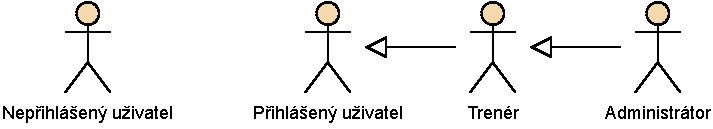
\includegraphics[width=0.9\textwidth]{images/actors.pdf}
\end{figure}

\subsection{Případy užití}
\begin{enumerate}[label=\textcolor{decoration}{\textbf{UC\arabic*}}, leftmargin=1cm, align=left, labelwidth=8mm]

	\myItem{registrace}
	Před~prvním přístupem do~systému se musí člen klubu zaregistrovat. 
	\begin{enumerateNumbers}
		\item Nepřihlášený uživatel klikne na~položku \emph{Registrace} v~hlavní nabídce.
		\item Pro~úspěšné dokončení registrace musí vyplnit svou e-mailou adresu, registrační číslo, heslo, jméno a~příjmení a~kliknout na~tlačítko \emph{Registrovat}.
		\item Registraci musí následně schválit některý z~administrátorů a~poté se již nepřihlášený uživatel může pomocí zadaného registračního čísla a~hesla přihlásit do~systému.
	\end{enumerateNumbers}
	\newpage

	\myItem{přihlášení a~odhlášení z~aplikace}
	Nepřihlášený uživatel bude při~pokusu o~přístup do~systému vyzván k~přihlášení.
	\begin{enumerateNumbers}
		\item Nepřihlášený uživatel zadá své registrační číslo a~heslo a~klikne na~tlačítko \emph{Přihlásit}.
		\item Pokud přihlášení proběhlo úspěšně, bude uživatel přesměrován na~hlavní stránku aplikace nebo~na~stránku, na~kterou se snažil před~přihlášením přistoupit.
		\item Přihlášený uživatel má naopak možnost se ze~systému odhlásit kliknutím na~položku \emph{Odhlásit} v~hlavní nabídce.
	\end{enumerateNumbers}

	\myItem{zobrazení seznamu závodů nebo tréninků\label{uc:listevents}}
	Tento případ užití popisuje zobrazení seznamu závodů/tréninků evidovaných v~systému.
	\begin{enumerateNumbers}
		\item Přihlášený uživatel klikne na~položku \emph{Závody} nebo \emph{Tréninky} v~hlavní nabídce.
		\item Ve~výchozím nastavení se zobrazují všechny nadcházející události, avšak upravením filtru v~horní části stránky lze zobrazit i~minulé události nebo~provést filtraci na~základě názvu události.
		\item Na~jedné stránce se vždy zobrazuje maximální 15~událostí, další události je možné zobrazit přejitím na~následující (předchozí) stránku.
	\end{enumerateNumbers}

	\myItem{zobrazení detailních informací o~události\label{uc:eventdetail}}
	V~seznamu závodů/tréninků jsou zobrazovány pouze základní informace, pro~zobrazení detailních informací o události je nezbytné přejít na~samostatnou stránku.
	\begin{enumerateNumbers}
		\item Přihlášený uživatel se může prokliknout na~stránku s~informacemi o~události z(e):
		\begin{enumerate}[label=\textcolor{decoration}{\textbf{\alph*.}}]
			\item seznamu závodů/tréninků (viz~\ref{uc:listevents}).
			\item hlavní stránky, kde se zobrazuje 5~závodů a 3 tréninky, u~kterých nejdříve končí uzávěrka přihlášek.
		\end{enumerate}
		\item Přechod na~stránku se~všemi evidovanými informacemi o~události proběhne po~kliknutí na~název události v~jednom ze~seznamů uvedených výše.
	\end{enumerateNumbers}

	\myItem{přihlášení na~událost}
	Přihlášení na~událost je možné provést pouze pokud událost nebyla zrušena, neproběhla uzávěrka přihlášek a~pokud již není daný uživatel na~danou událost přihlášený.
	\begin{enumerateNumbers}
		\item Přihlášený uživatel přejde na~stránku s~detailními informacemi o~události (viz~\ref{uc:eventdetail}).
		\item Uživatel vybere jednu z~nabízených kategorií a~volitelně sdělí, zda má možnost jet vlastním autem a~svézt s~sebou i~další členy klubu.
		\item Účast na~události potvrdí uživatel kliknutím na~tlačítko \emph{Přihlásit}.
	\end{enumerateNumbers}

	\myItem{odhlášení z~události}
	Odhlášení z~události je možné provést pouze pokud nebyla událost zrušena, neproběhla uzávěrka přihlášek a~pokud je daný uživatel na~danou událost přihlášený.
	\begin{enumerateNumbers}
		\item Přihlášený uživatel přejde na~stránku s~detailními informacemi o~události (viz~\ref{uc:eventdetail}).
		\item Účast na~události uživatel odřekne kliknutím na~tlačítko \emph{Odhlásit} a potvrzením následně zobrazeného dialogu.
	\end{enumerateNumbers}
	\newpage

	\myItem{přidání a~úprava komentáře}
	Tento případ užití popisuje přidání a~následnou úpravu komentáře u~konkrétní události.
	\begin{enumerateNumbers}
		\item Přihlášený uživatel přejde na~stránku s~detailními informacemi o~události (viz~\ref{uc:eventdetail}).
		\item Po~napsání komentáře do~textového pole klikne na~tlačítko \emph{Přidat komentář}.
		\item Své komentáře má uživatel možnost upravit kliknutím na~ikonku pro~úpravu vedle konkrétního komentáře. To načte napsaný komentář do~textového pole a~po~jeho úpravě dojde k~uložení kliknutím na~tlačítko \emph{Upravit komentář}.
	\end{enumerateNumbers}

	\myItem{úprava osobních údajů}
	Přihlášený uživatel si může změnit svou e-mailovou adresu a heslo, pomocí něhož se přihlašuje do systému.
	\begin{enumerateNumbers}
		\item Přihlášený uživatel klikne na~položku \emph{Nastavení} v~hlavní nabídce.
		\item Po~upravení požadovaných údajů klikne na~tlačítko \emph{Uložit změny}.
	\end{enumerateNumbers}

	\myItem{přidání události}
	Tento případ užití popisuje přidání nové události do~systému.
	\begin{enumerateNumbers}
		\item Trenér klikne na~položku \emph{Administrace} v~hlavní nabídce a~následně vybere možnost \emph{Přidat nový trénink} nebo \emph{Přidat nový závod}.
		\item Pokud je přidávaná událost již evidovaná v~IS~ORIS, může uživatel zadat ORIS~ID události a~většina požadovaných informací se automaticky předvyplní.
		\item Po~(do)vyplnění požadovaných informací se událost přidá do~systému kliknutím na~tlačítko \emph{Přidat událost}.
	\end{enumerateNumbers}

	\myItem{úprava události}
	Tento případ užití popisuje proces upravení události již evidované v~systému.
	\begin{enumerateNumbers}
		\item Trenér klikne na~položku \emph{Administrace} v~hlavní nabídce a~následně vybere ze~seznamu událost, kterou si přeje upravit.
		\item Po~upravení požadovaných informací klikne na~tlačítko \emph{Upravit událost}.
	\end{enumerateNumbers}

	\myItem{synchronizace přihlášek}
	Role trenér v~tomto systému sama o~sobě nestačí pro~odeslání přihlášek do~IS~ORIS. Je zapotřebí, aby uživatel měl také zřízený účet v~IS~ORIS a~měl práva na~přihlašování závodníků klubu.
	\begin{enumerateNumbers}
		\item Trenér klikne na~položku \emph{Administrace} v~hlavní nabídce a vybere závod, jehož přihlášky si přeje odeslat.
		\item Přihlášky evidované u~dané události budou odeslány po vyplnění přístupových údajů do~IS~ORIS a~kliknutí na~tlačítko \emph{Odeslat přihlášky}.
	\end{enumerateNumbers}

	\myItem{vytvoření a úprava oznámení}
	Tento případ užití popisuje vytvoření a úpravu oznámení.
	\begin{enumerateNumbers}
		\item Pro vytvoření nového oznámení klikne trenér na~položku \emph{Administrace} v~hlavní nabídce a~následně vybere možnost pro přidání nového oznámení.
		\item Oznámení bude uloženo po vyplnění formuláře a kliknutí na tlačítko \emph{Přidat oznámení}.
		\item Úpravu existujícího oznámení je naopak možné provést po vybrání konkrétního oznámení v administraci a kliknutí na tlačítko \emph{Upravit vybrané oznámení}.
		\item Provedené změny budou uloženy po kliknutí na~tlačítko \emph{Upravit oznámení}.
	\end{enumerateNumbers}

	\myItem{úprava a anonymizace uživatele}
	Funkce anonymizace uživatele přenastaví členovo jméno na~\emph{Anonymní uživatel} a~smaže všechny jeho údaje (registrační číslo, stav osobního konta, typ členství, e-mail a~heslo). Tímto je uživateli znemožněno přihlášení do~aplikace.
	\begin{enumerateNumbers}
		\item Administrátor klikne na~položku \emph{Administrace} v~hlavní nabídce a~následně vybere ze~seznamu uživatele, kterého si přeje upravit nebo anonymizovat.
		\item Anonymizaci člena lze provést kliknutím na~tlačítko \emph{Anonymizovat vybraného člena} a potvrzením následně zobrazeného dialogu.
		\item Formulář pro úpravu uživatele se naopak zobrazí po kliknutí na tlačítko \emph{Upravit vybraného člena}. Po~upravení požadovaných informací se změny uloží kliknutím na~tlačítko \emph{Uložit změny}.
	\end{enumerateNumbers}

\end{enumerate}

\subsection{Pokrytí funkčních požadavků v případech užití}
V~tabulce \ref{table:use-cases} je zachyceno pokrytí funkčních požadavků v~jednotlivých případech užití. Symbol~\Checkmark říká, že příslušný funkční požadavek je součástí daného případu užití.

\begin{table}[h]
	\centering
	\caption{\label{table:use-cases}Mapování funkčních požadavků na~případy užití}
	\begin{tabularx}{0.95\textwidth}{|C||C|C|C|C|C|C|}
		\hline
			 & F1 & F2 & F3 & F4 & F5 & F6            \\ \hline\hline
		UC1  & \Checkmark &    &    &    &    &       \\ \hline
		UC2  & \Checkmark &    &    &    &    &       \\ \hline
		UC3  &    & \Checkmark &    &    &    &       \\ \hline
		UC4  &    & \Checkmark &    &    &    &       \\ \hline
		UC5  &    &    & \Checkmark &    &    &       \\ \hline
		UC6  &    &    & \Checkmark &    &    &       \\ \hline
		UC7  &    &    &    &    &    & \Checkmark    \\ \hline
		UC8  & \Checkmark &    &    &    &    &       \\ \hline
		UC9  &    & \Checkmark &    &    &    &       \\ \hline
		UC10 &    & \Checkmark &    &    &    &       \\ \hline
		UC11 &    &    &    & \Checkmark &    &       \\ \hline
		UC12 &    &    &    &    & \Checkmark &       \\ \hline
		UC13 & \Checkmark &    &    &    &    &       \\ \hline
	\end{tabularx}
\end{table}
